%\subsection{تخمین پارامتر کانال یاو}
%برای اصلاح پارامترهای یاو چندین آزمایش انجام شد و با استفاده از داده‌های ثبت شده از وضعیت استند در کانال پیچ  و جعبه‌ابزار
%\lr{Parameter Estimator}
%پارامترها اصلاح شدند.
%برای آزمایش یاو همه‌ی موتورها با دور مختلف شروع به حرکت کردند و از خروجی‌ سنسور داده برداری شد. سپس، مدل و پارامترهای داده‌های ثبت شده‌ی سنسور (وضعیت استند در کانال یاو) به جعبه‌ابزار
%\lr{Parameter Estimator}
%داده شد. نتایج آزمایش‌های کانال یاو بعد از اصلاح پارامترها در شکل
%\ref{yaw_ps1} و \ref{yaw_ps2}
%آورده شده است.

%\begin{figure}[H]
%	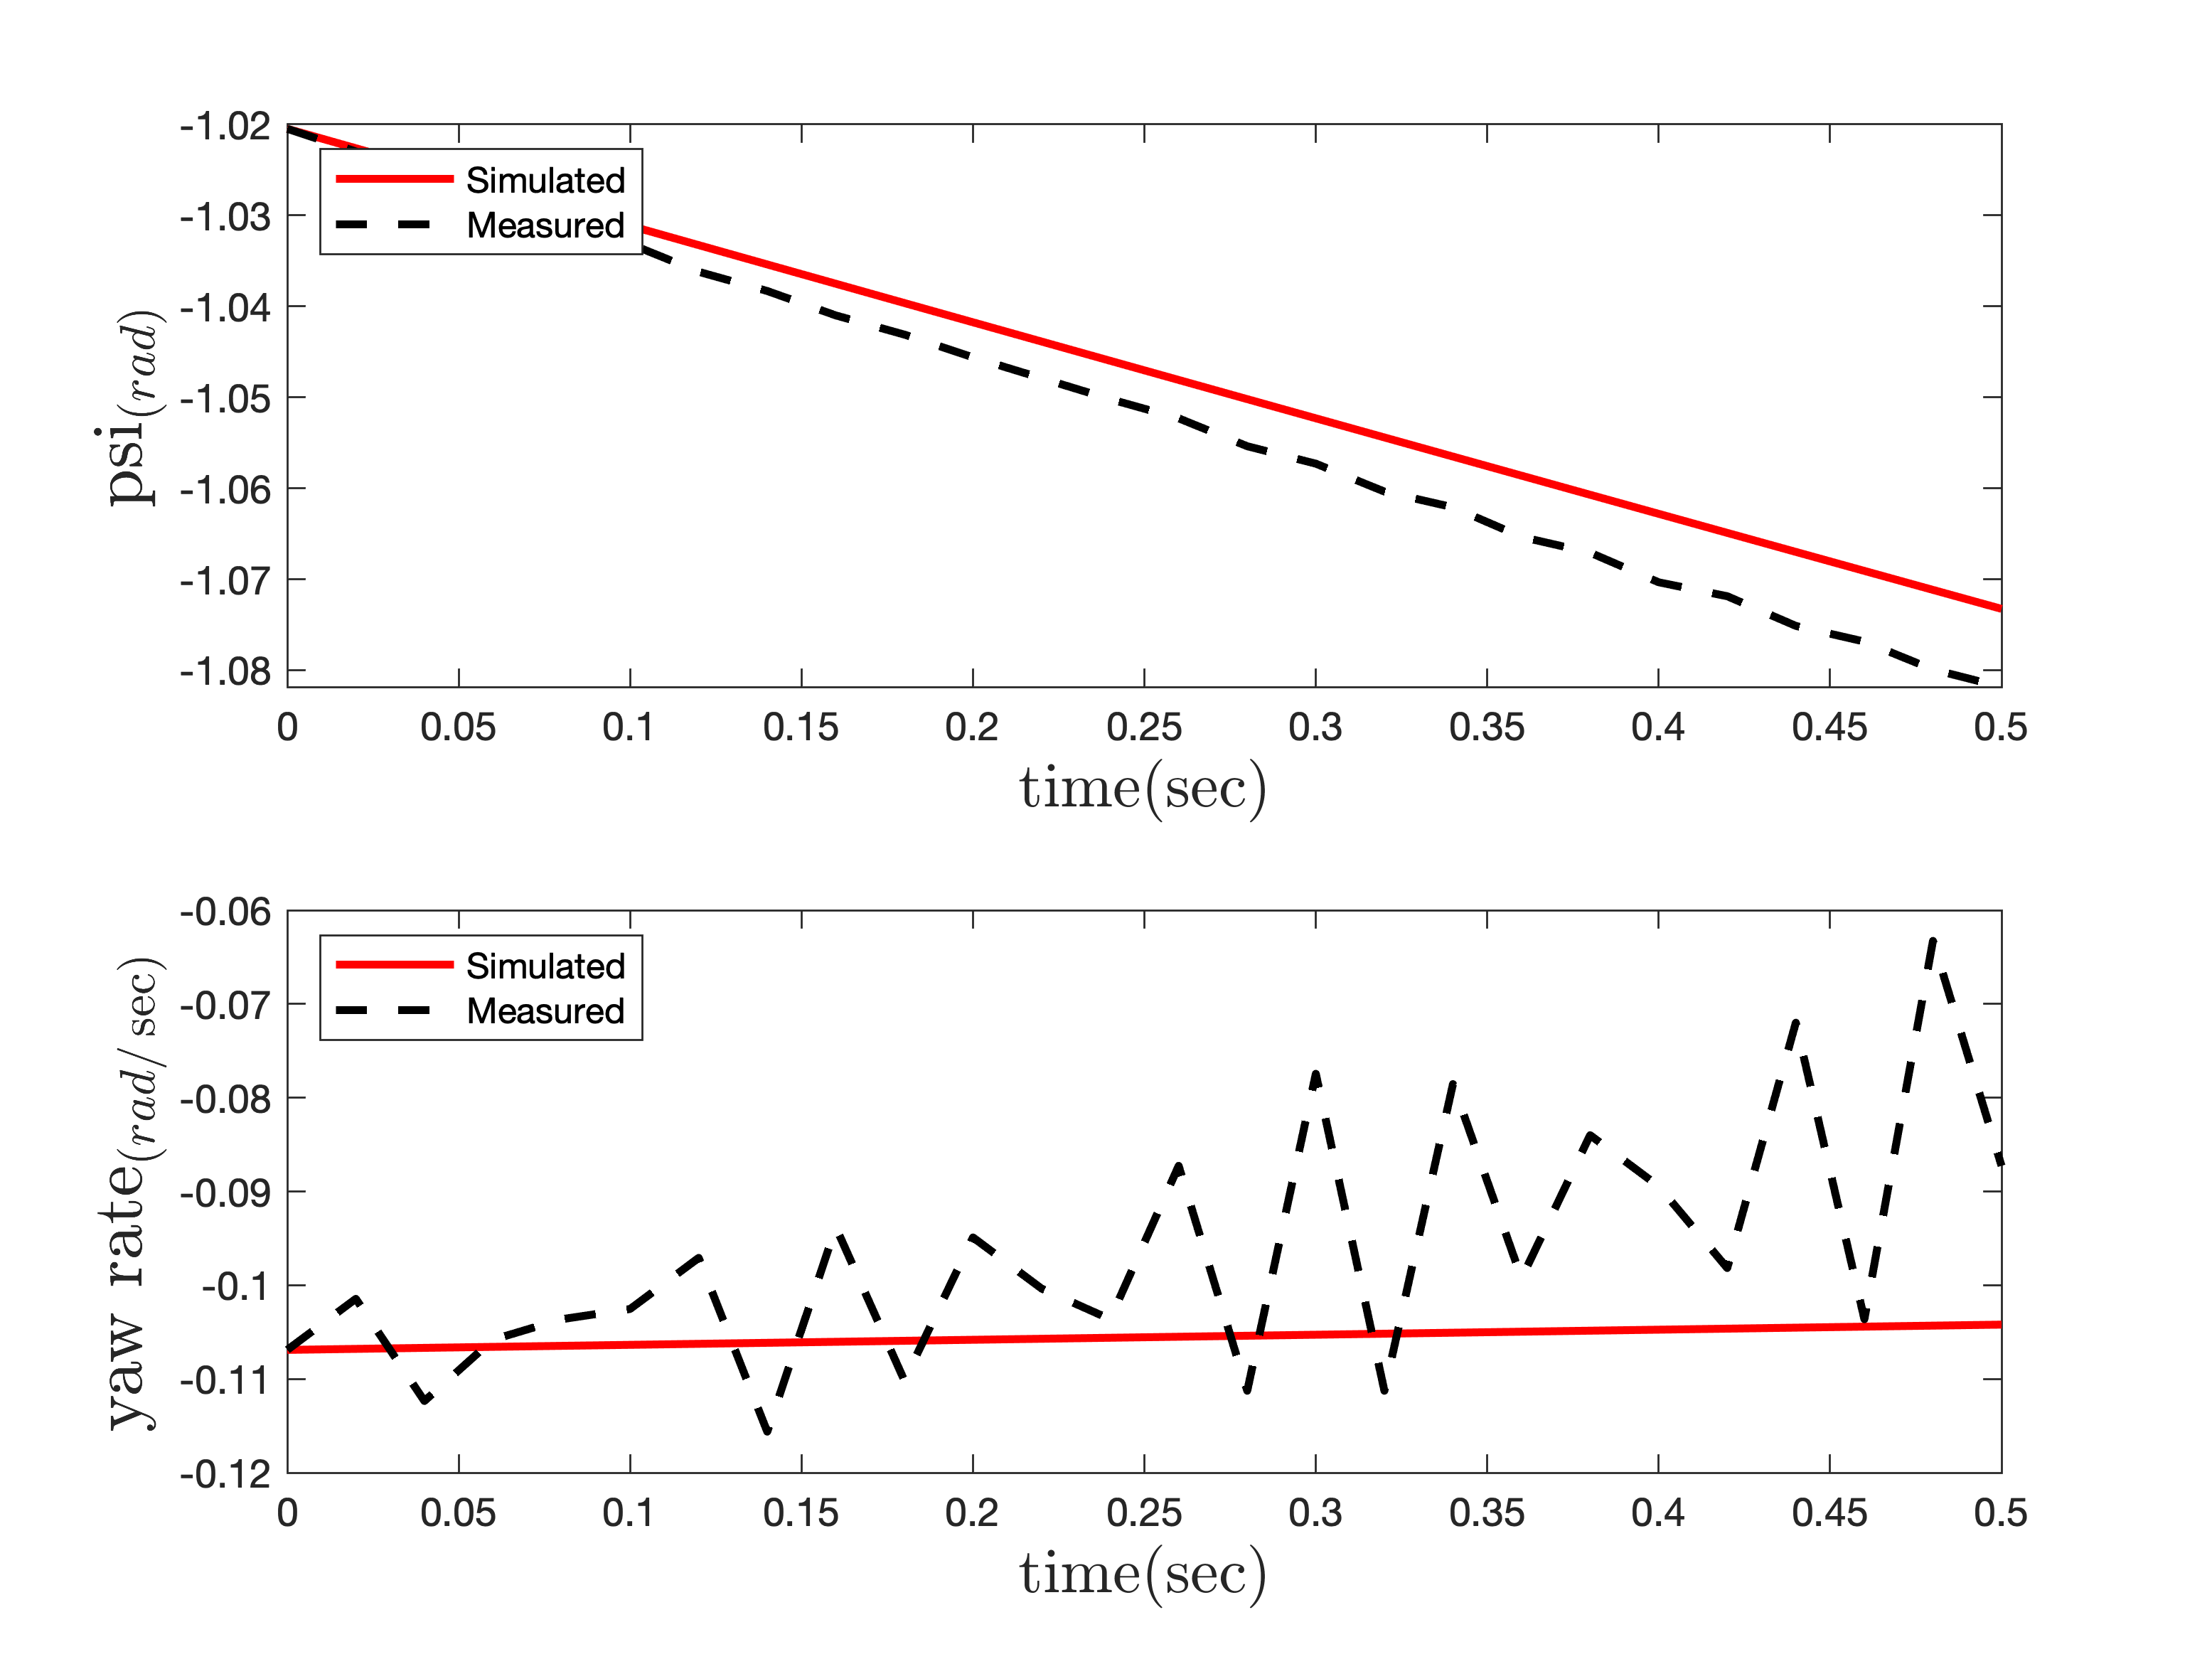
\includegraphics[width=12cm]{../Figures/RCP/yaw_parameter_estimation/RCP_yaw_S1.png}
%	\centering
%	\caption{مقايسه وضعیت استند در  آزمايش اول و شبیه‌سازی، پس از تخمین پارامترهای کانال یاو}
%	\label{yaw_ps1}
%\end{figure}
مقایسه وضعیت شبیه‌سازی و واقعیت چهارپره در کانال یاو و پارامترهای اصلاح شده آورده شده‌است.



\begin{minipage}[H]{\linewidth}
	\hfill
	\begin{minipage}[b]{0.49\linewidth}
		\centering
		\begin{tabular}{ccc}\hline
			پارامتر & مقدار پارامتر  & مقدار پارامتر بعد از اصلاح
			\\ \hline
			$C_2$  & $5.45\times10^{-5}$ & $1.3\times10^{-5}$ \\
			$C_3$  & $0.014$ & $0.017$ \\
			\\\\\\
		\end{tabular}
		\captionof{table}{مقايسه پارامترهای کانال یاو قبل و بعد از اصلاح}
	\end{minipage}
	\begin{minipage}[b]{0.48\linewidth}
		\centering
		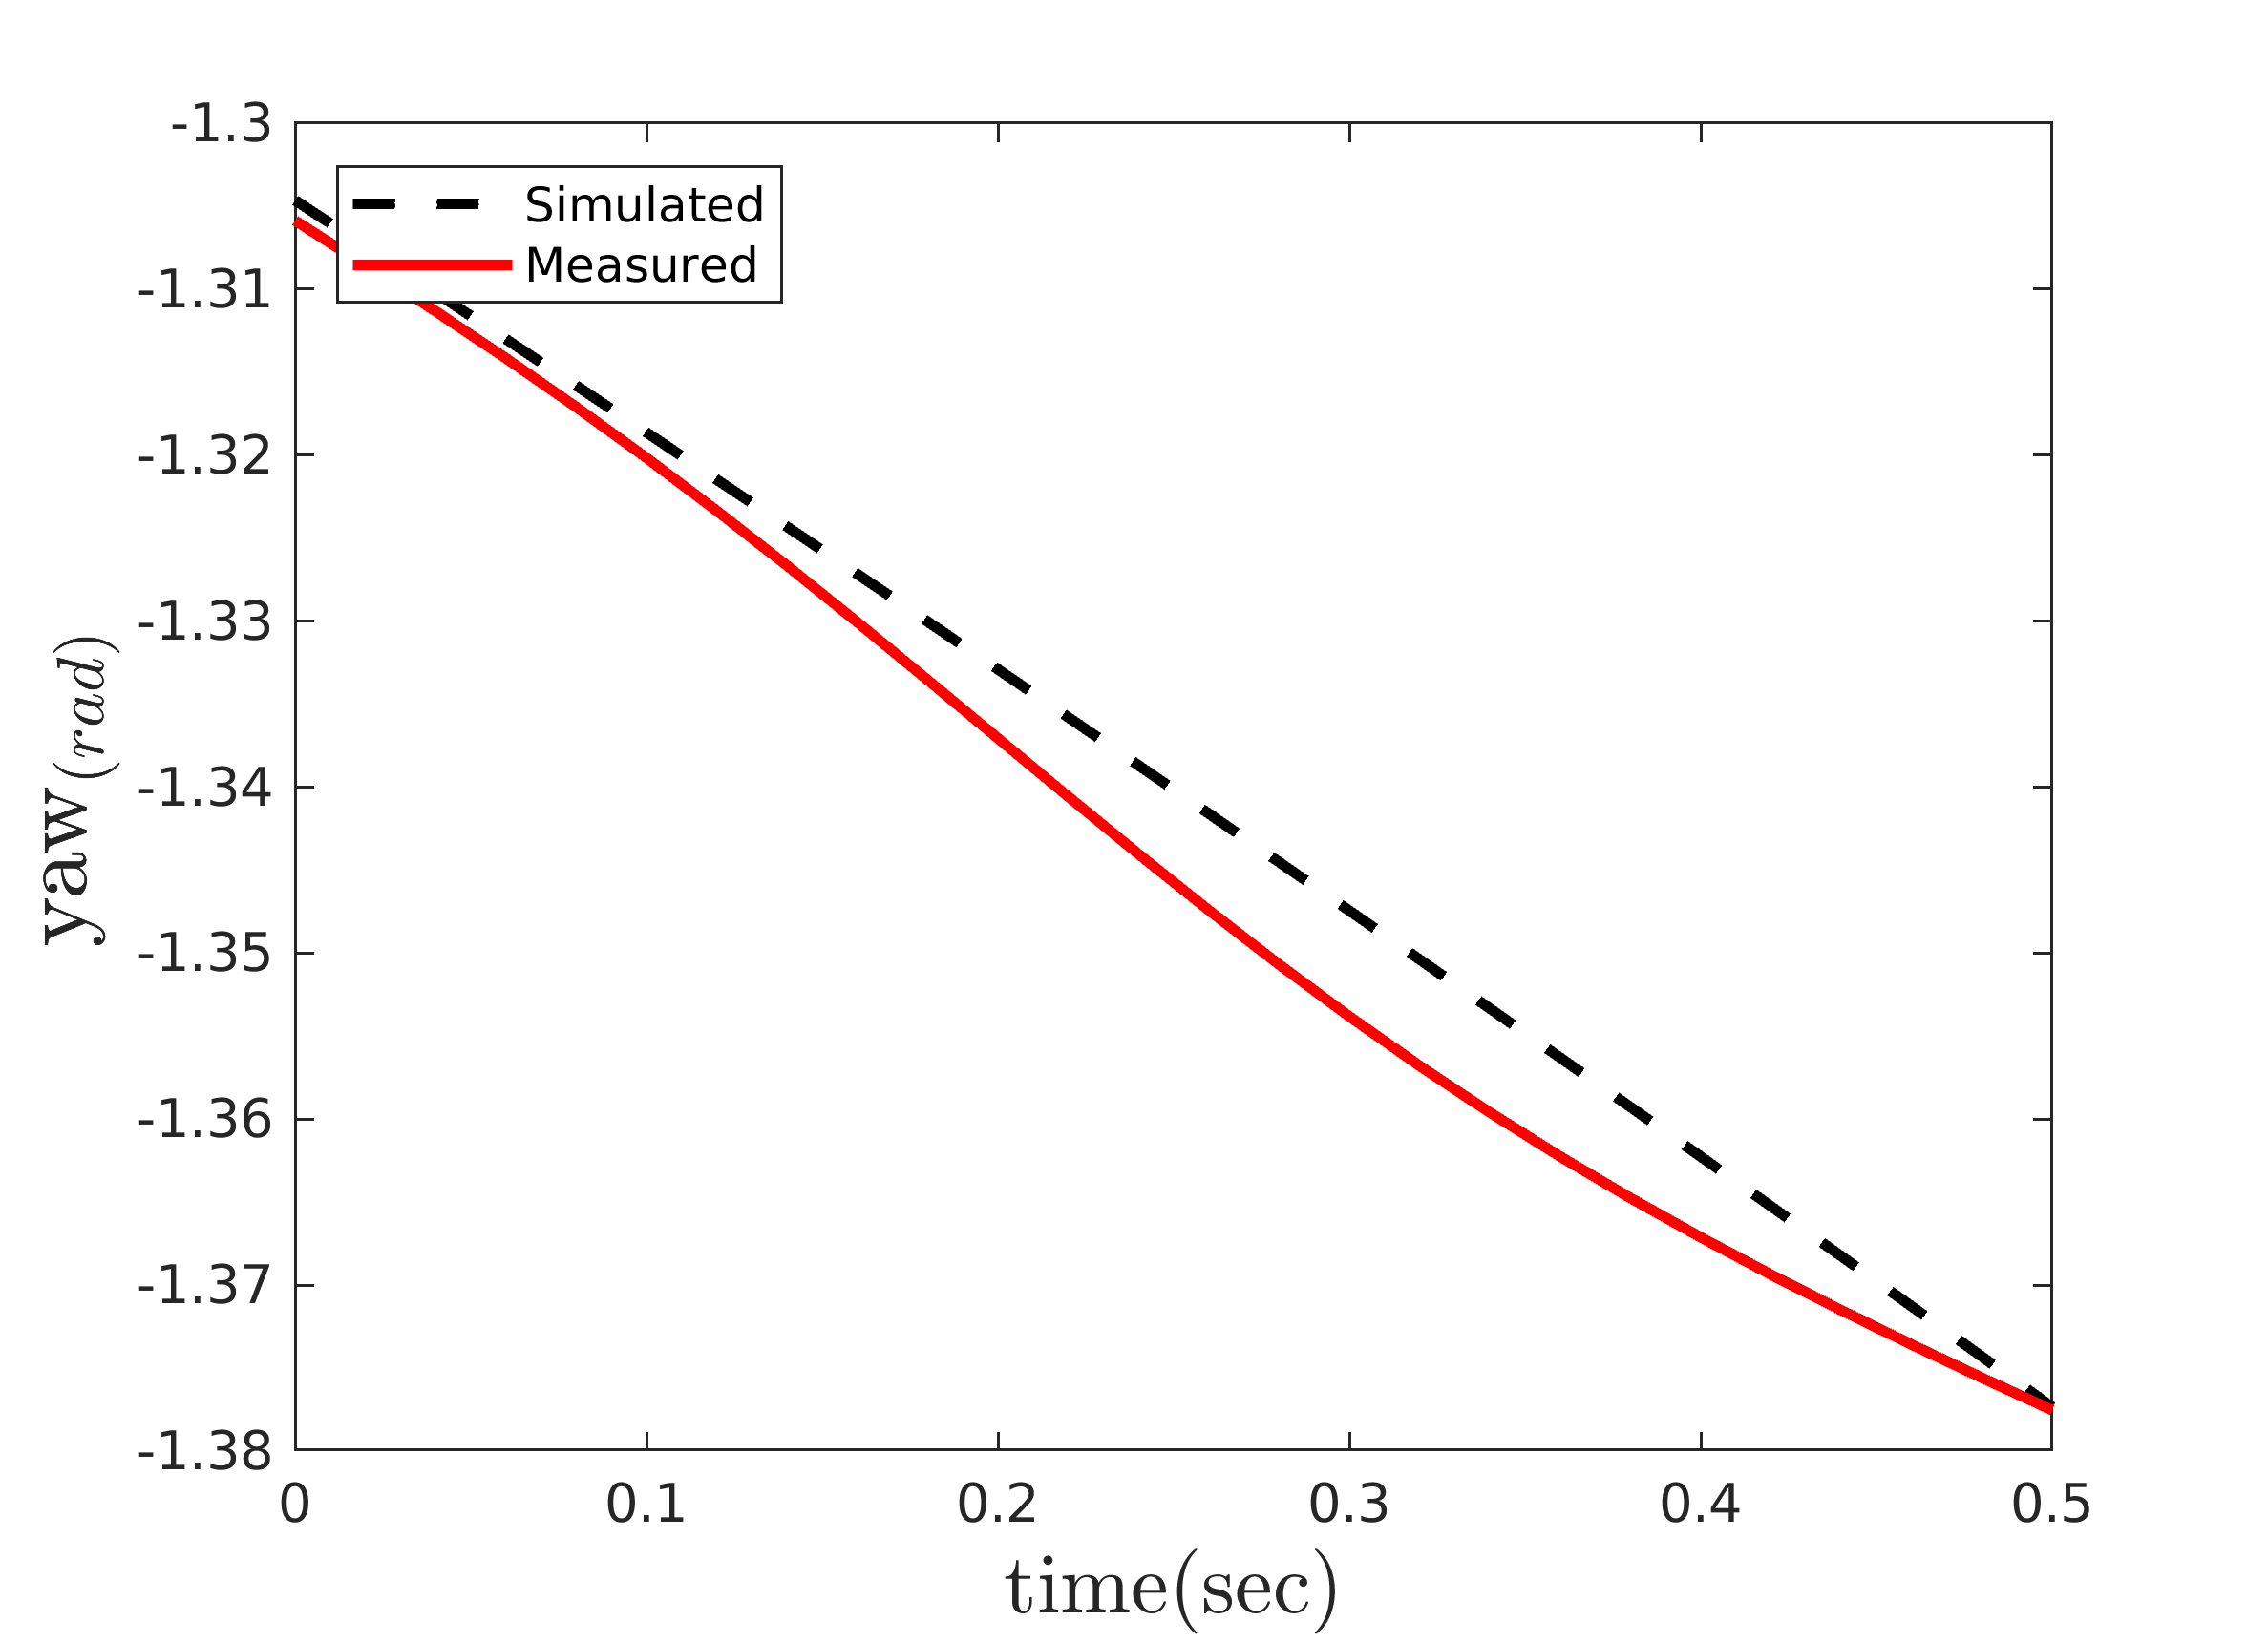
\includegraphics[width=1\linewidth]{../Figures/RCP/yaw_parameter_estimation/RCP_yaw_S2.png}
		\captionof{figure}{مقايسه وضعیت کانال یاو در شبیه‌سازی و واقعیت}
	\end{minipage}
\end{minipage}
%\begin{figure}[H]
%	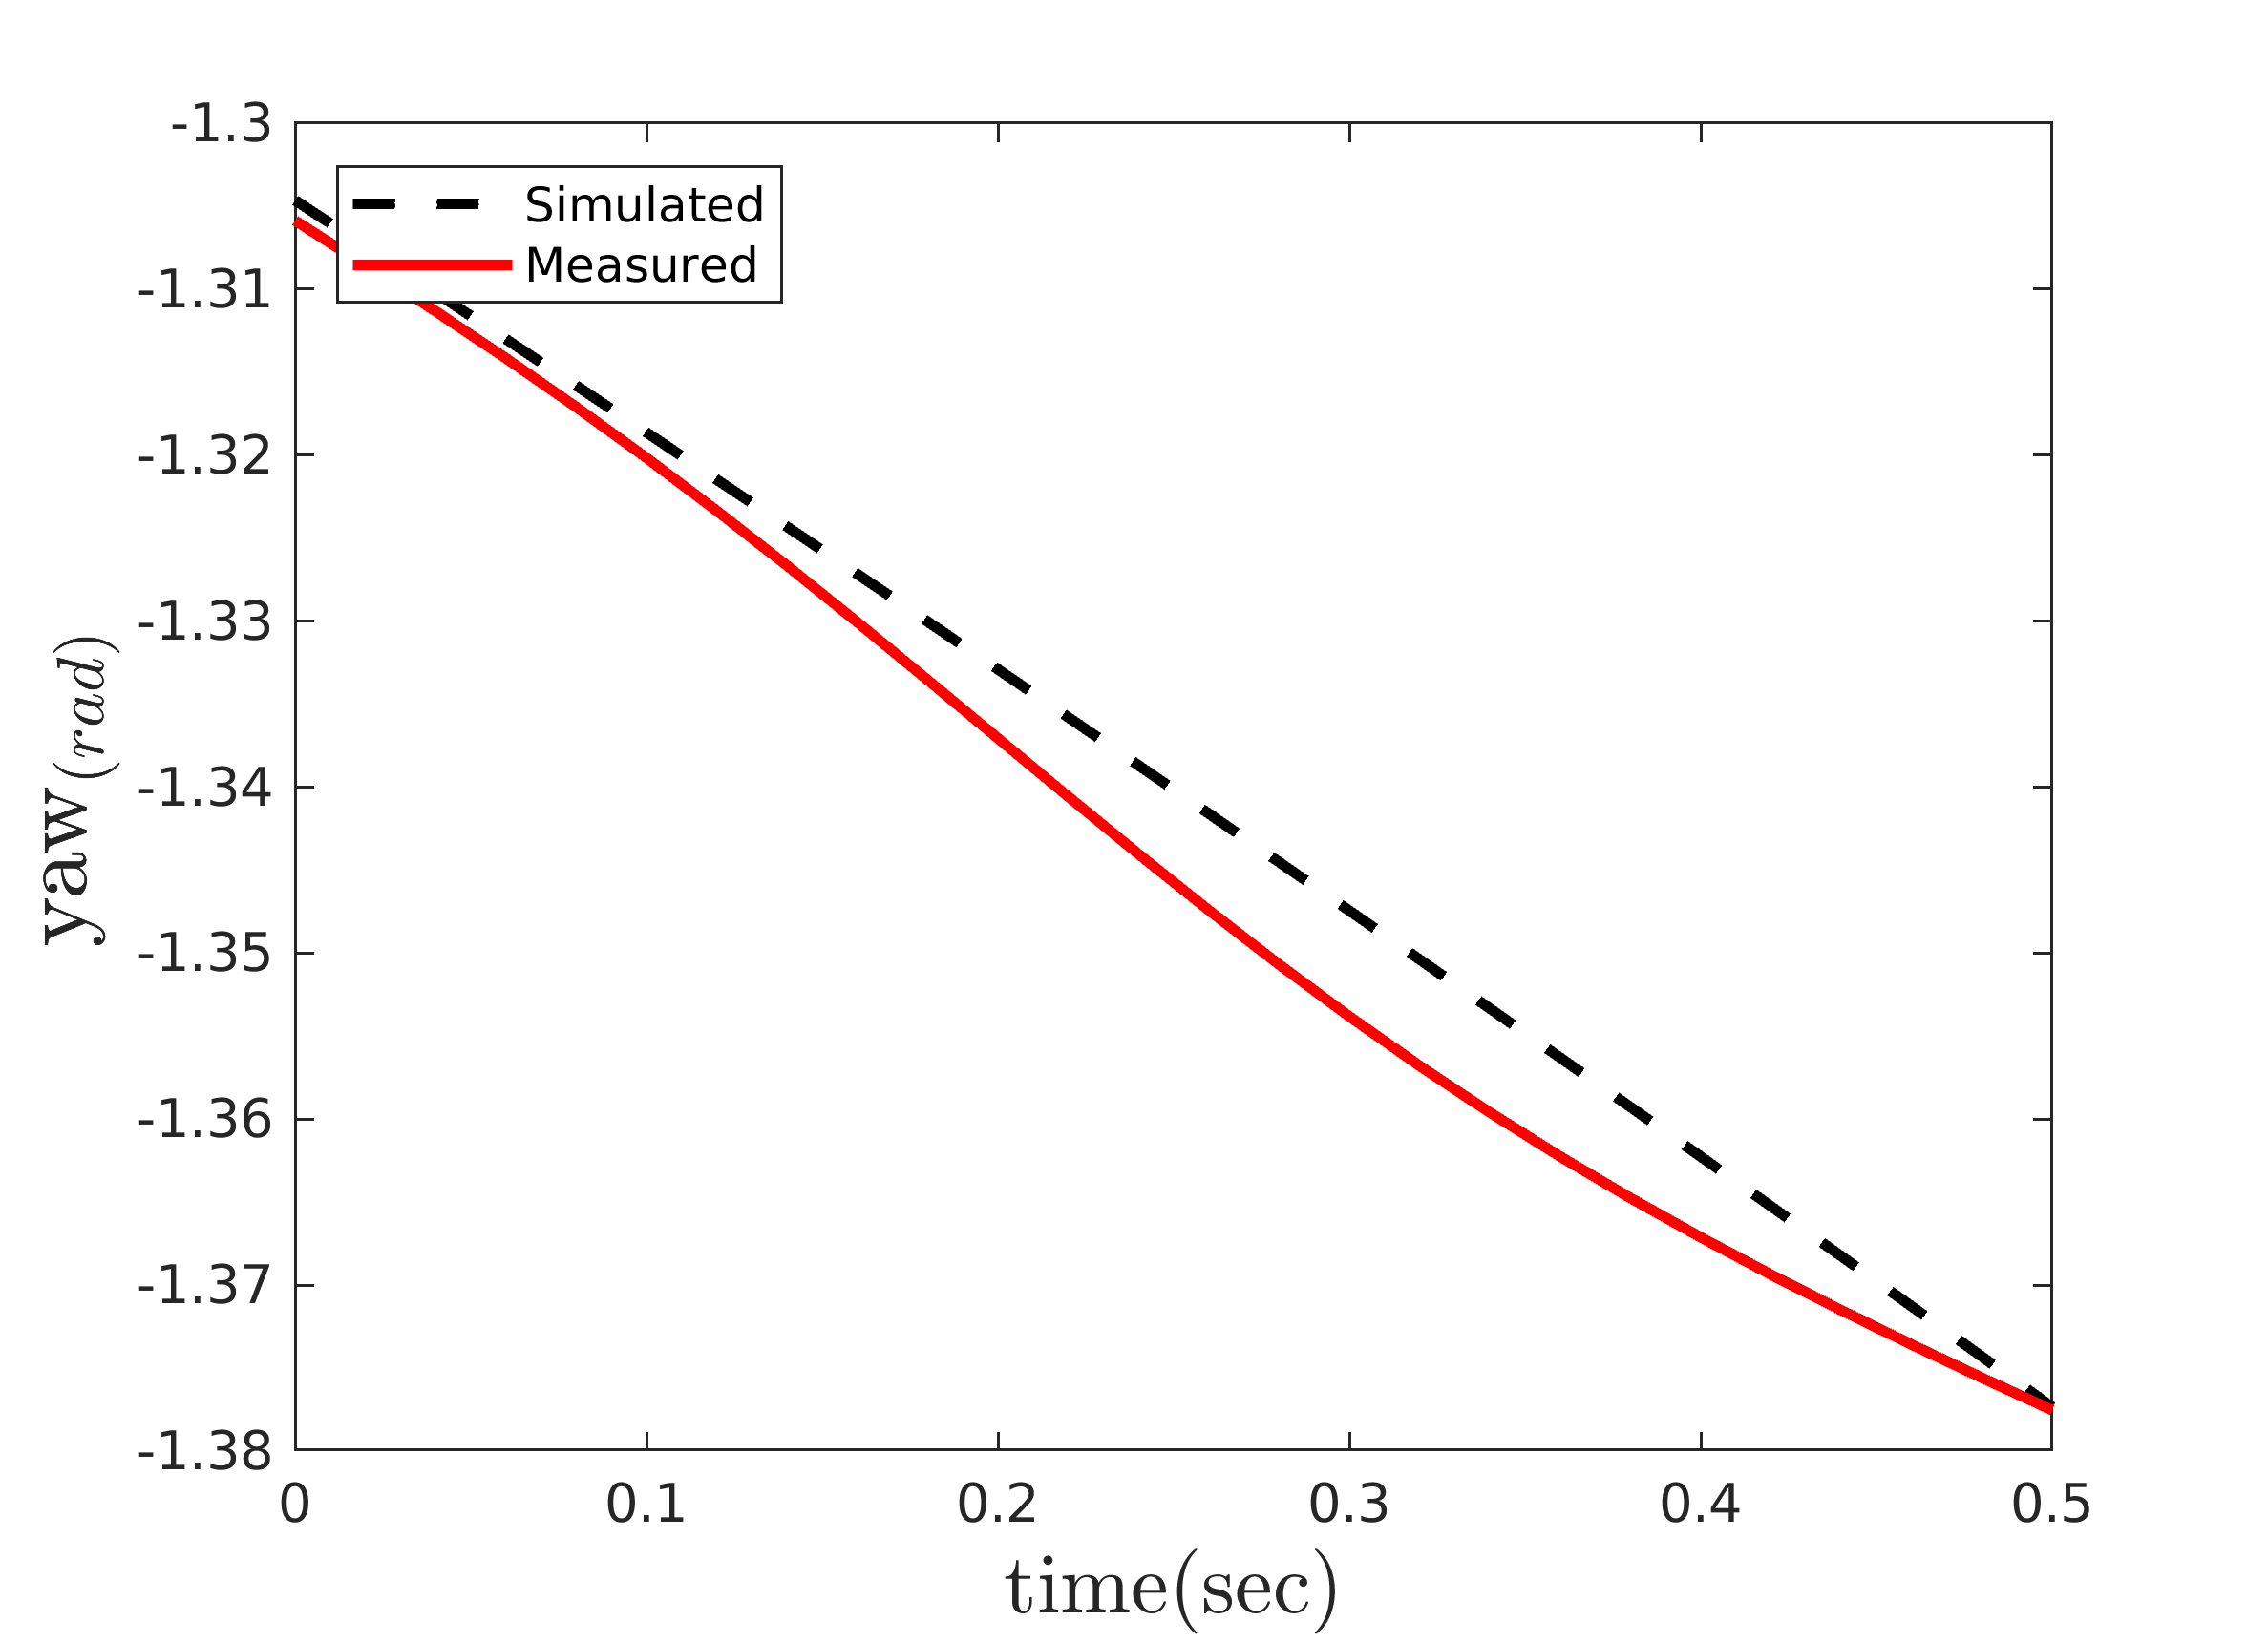
\includegraphics[width=.48\linewidth]{../Figures/RCP/yaw_parameter_estimation/RCP_yaw_S2.png}
%	\centering
%	\caption{مقايسه  وضعیت استند در  آزمايش دوم و شبیه‌سازی، پس از تخمین پارامترهای کانال یاو}
%	\label{yaw_ps2}
%\end{figure}